\section{Introduction}

\begin{frame}[fragile]{Last Week}
	\begin{columns}[onlytextwidth]
		\column{.4\textwidth}
		
		\begin{itemize}
			\item Have admiration for him
			\item 
			\item 
		\end{itemize}
		
		\column{.6\textwidth}
		
		\begin{figure}
			
\includegraphics[width=.5\linewidth]{peifu.jpg}
		\end{figure}
		
	\end{columns}
\end{frame}


\begin{frame}[fragile]{Last Week}
	\begin{columns}[onlytextwidth]
		\column{.4\textwidth}
		
		\begin{itemize}
			\item Have admiration for him
			\item Confused
			\item 
		\end{itemize}
		
		\column{.6\textwidth}
		
		\begin{figure}
			
\includegraphics[width=.5\linewidth]{mengbi.jpg}
		\end{figure}
		
	\end{columns}
\end{frame}

\begin{frame}[fragile]{Last Week}
	\begin{columns}[onlytextwidth]
		\column{.4\textwidth}
		
		\begin{itemize}
			\item Have admiration for him
			\item Confused
			\item In Despair
		\end{itemize}
		
		\column{.6\textwidth}
		
		\begin{figure}
			
\includegraphics[width=.5\linewidth]{juewang.jpg}
		\end{figure}
		
	\end{columns}
\end{frame}



\begin{frame}[fragile]{Story About Adversarial training}
	\begin{columns}[onlytextwidth]
		\column{.4\textwidth}
		
		\begin{figure}
			\caption{Dog}
			
\includegraphics[height=0.5\textheight]{fig0.jpg}
		\end{figure}
	
		\column{.5\textwidth}
		\begin{figure}
			\caption{What?}
			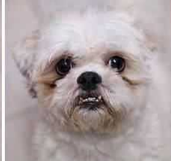
\includegraphics[height=0.5\textheight]{fig2.jpg}
		\end{figure}
	
		\end{columns}
		\begin{itemize}
			\item Why?
		\end{itemize}
				
		

\end{frame}
\begin{frame}[fragile]{Story About Adversarial training}
	\begin{columns}[onlytextwidth]
		\column{.3\textwidth}
		\begin{figure}
			\caption{Dog}
			
\includegraphics[height=0.5\textheight]{fig0.jpg}
		\end{figure}
		\column{.3\textwidth}
		\begin{figure}
			\caption{Noise}
			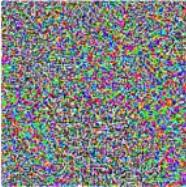
\includegraphics[height=0.5\textheight]{zy.jpg}
		\end{figure}
		\column{.3\textwidth}
		\begin{figure}
			\caption{What?}
			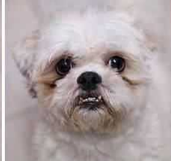
\includegraphics[height=0.5\textheight]{fig2.jpg}
		\end{figure}
		
	\end{columns}
	\begin{itemize}
		\item perturbations
	\end{itemize}
	
	
	
\end{frame}

\begin{frame}[fragile]{NonLinear}
	
	\begin{columns}[onlytextwidth]
		\column{1\textwidth}
		\begin{figure}

			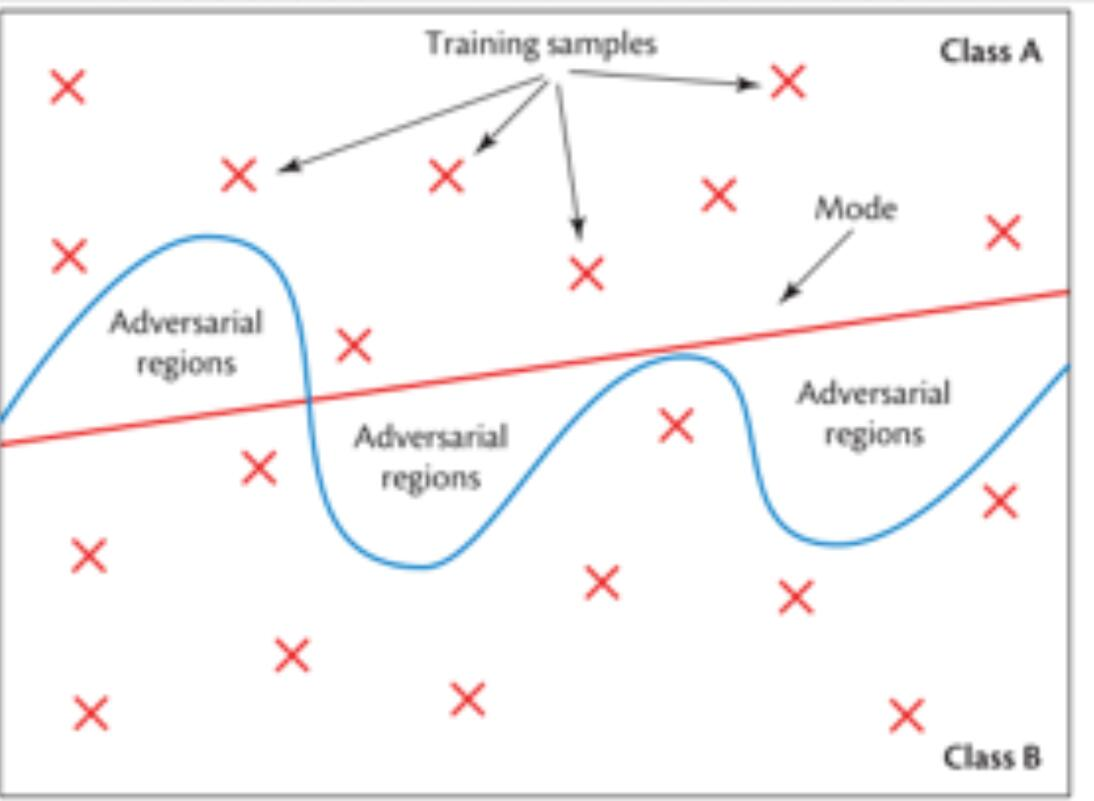
\includegraphics[height=.8\textheight]{exp1.jpg}
		\end{figure}

		
	\end{columns}
	
	
	
\end{frame}

\begin{frame}[fragile]{Linear Behavior}

\begin{itemize}
	\item The precision of an individual input feature is limited
	\item Example: 8 bits per pixel \& 1/255 of the dynamic
	range
	\item for the classifier to respond differently to an input $x$ than to an adversarial input $\widetilde{x}= x + \eta $ if every element of the perturbation $\eta$ is smaller than the precision of the features
	
\end{itemize}



\end{frame}

